\section{A Model of Third-Party Software Library Adoption (RQ1)}
We describe a software library adoption model in the industry that we derived based on our interviews with 24 software practitioners from the industry. Since developers are consumers of libraries and we outlined their behavior model during the library adoption process, we named the model \model.

%The model is composed of five attributes of a suite of conditions, factors, information sources, challenges, and \principle\space that influence the lifecycle of library adoption. 

% To explain the model, we divide RQ1 in 7 sub-RQs:

% \nd\bf{RQ1.1:} What behavior model developers follow while adopting libraries?

% \nd\bf{RQ1.2:} What are the process developers follow in the industry during their adoption of a software library?

% \nd\bf{RQ1.3:} What are the major data sources developers use during their adoption decision of a software library?

% \nd\bf{RQ1.4:} What conditions influence the library adoption process?

% \nd\bf{RQ1.5:} What library specific technical factors developers consider during the library adoption process?

% \nd\bf{RQ1.6:} What challenges developers face while adopting software libraries

% \nd\textbf{RQ1.7:} What \principle\space do developers follow during the library adoption process?


\begin{figure*}
    \centering
    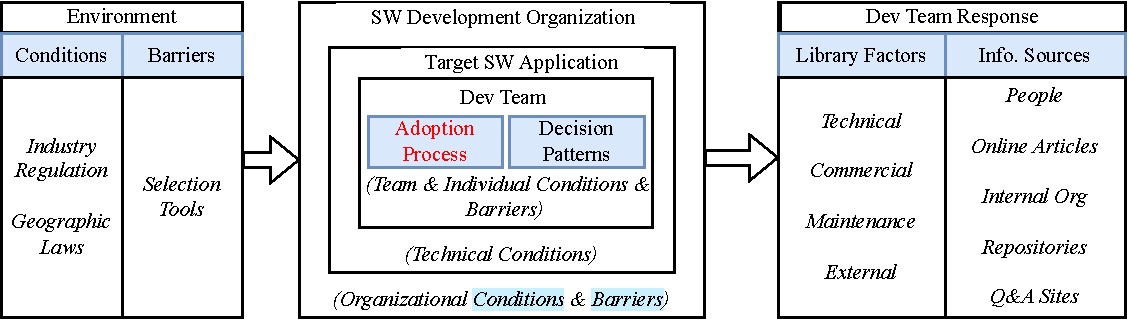
\includegraphics[scale=0.8  ]{images/Library-adoption-framework.v4.pdf}
    \caption{Conceptual framework of the library consumer behavior model. Example concepts are shown in \textit{italic}.}
    \label{fig:framework}
\end{figure*}

\begin{figure*}
    \centering
    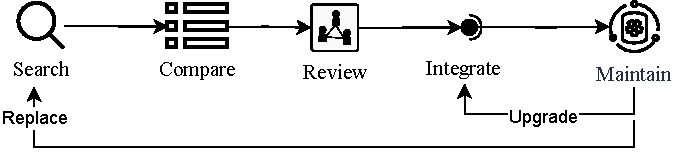
\includegraphics[scale=0.8  ]{images/Library-selection-process.pdf}
    \caption{Steps and life cycle of library adoption process}
    \label{fig:selection-process}
\end{figure*}
%\subsection{The Adoption Model and Dimensions}\label{sec:rq1}
%\subsection{Library Consumer Behavior Model}\label{sec:framework}
%\subsubsection{The Model} 

The {\model} consists of three building blocks as shown in Figure \ref{fig:framework}, the external environments (i.e., external conditions and barriers), the internal context comprising barriers, conditions, processes, and decision patterns based on the organization, the development team, and even the individual developers, and finally, the development team's response (for considering specific library specific factors or information sources) influenced by the first two blocks (external and internal attributes). 
At the center of the model resides the adoption process, which is used to select and adopt a software library. The process consists of a set of steps, each completed in order as shown in Figure \ref{fig:selection-process}. 

% The completion of the steps is supported by consultation with different information sources. The process is influenced by a suite of conditions, factors, and \principle. Figure~\ref{fig:framework} visualizes the relationships between the selection process, conditions, factors, sources, and the \principle. 


% We find that developers seek support for their evaluation from a variety of sources, which are included in the pattern as support. The categories of support are:
% \begin{inparaenum}[(S1)] 
% \item known people, 
% \item search engine and online articles, 
% \item internal organizational sources, 
% \item repositories, and 
% \item community question-answer sites.
% \end{inparaenum} 
% Support is detailed in section~\ref{sec:sources}.

Under complex organizational contexts, developers tend to follow certain {\principle} (knowingly or unknowingly) to extract the right benefits and to tackle the disadvantages of the libraries throughout the whole adoption process. For example, on the basis of the {\principle}, they can skip or include certain steps such as \code{review} or \code{maintain} may be skipped under \code{Just Do It} pattern. 
Hence, {\principle} became the central theme of the library adoption process. The other aspects of the library adoption process are conditions, factors, and information sources.  

% The software library adoption process has five major steps, during which factors are considered and information is sought. The steps are:
% \begin{inparaenum}[(P1)] 
% \item information search, 
% \item comparison of short-listed libraries, 
% \item review of decision, 
% \item integration into application, and finally 
% \item life-long maintenance.
% \end{inparaenum} 
% These are discussed in more detail in section~\ref{sec:phases}. 
% One important aspect of the process is to recognize that there can be a return to earlier steps. That is, once a library has already been selected and integrated, new versions may necessitate returning to the integration phase. If a library becomes obsolete or is no longer a good fit, the need for replacement may trigger returning to the beginning of the process. The knowledge that upgrade and/or replacement may be necessary can affect how developers view the decision.

% There are conditions which influence the choice of guiding principle.  The five categories of conditions are:
% \begin{inparaenum}[(C1)] 
% \item environmental (external to the organization), 
% \item organizational, 
% \item team specific, 
% \item individual developer specific, and 
% \item particular technical situation. 
% \end{inparaenum} 
% We elaborate on conditions in section~\ref{sec:conditions}.


% Selection factors are the categories of considerations developers might consider when evaluating a library. Depending on the guiding principle, certain factors might be favored over others in the evaluation. The factors are:
% \begin{inparaenum}[(F1)] 
% \item technical software specific, 
% \item commercial supply chain, 
% \item support and maintenance, and 
% \item external factors outside the primary influence of libraries.
% \end{inparaenum} 
% Factors are elaborated in section \ref{sec:factors}.


% The six guiding principles central to the library adoption process are: 
% \begin{inparaenum}[(GP1)] 
% \item Just Do It, 
% \item Reuse Robust Component, 
% \item Maximize Flexibility, 
% \item Empower the Team, 
% \item Ensure Compliance, and
% \item Maintain Continuous Stability. 
% \end{inparaenum} 
% Guiding principles are described in greater detail in section~\ref{sec:gp}.



% While developers following on this principle can also ignore some library specific factors such as \code{license}, other developers would put serious emphasis on the same factor, if they are following \code{Ensure Compliance} principle. Based on the emphasis on the factors, their source of information also changes. For example, developers will have to consult with internal organizational sources if they care for \code{license} factor.

As we worked with the data, we had some insights. First, library adoption is not a one-off selection event, rather it has a complete process involving selection, integration, and post-integration maintenance. Secondly, in addition to all the benefits libraries offer, they also have disadvantages, such as legal risks with licenses and life-long upgrades of library versions. The benefits are seen in the following quote:
\qi{I have used many third-party libraries because they are ready-to-use tools, right? If I don't use them, I need to spend lots of time developing my own libraries to do like sometimes very simple stuff. I think it seems simple but when you get to the bottom of it, it will take time to do some let's say preprocessing or processing on the data that you have. But by using the third-party libraries you can just import it and use the functions and it's very easy to use and very fast and user friendly.}{P11}

Evidence of disadvantage is illustrated by the following quote:
 \qi{There can be flaws within the library that could introduce security flaws and attacks to your system. It is always, always risky when you build a core component on top of a library and the library is not getting developed.}{P15} 
 
In the following subsections, we present the major attributes of the {\model} process, sources, conditions, factors, barriers, and {\principle} which have 18, 17, 23, 28, 7, and 6 concepts respectively. For the sake of simplicity, we provide the taxonomy chart of concepts for the major attributes (process, sources, conditions, and factors) which have more than ten concepts. For the barriers and {\principle} attributes, we provide the description of all the internal concepts since they are lower in number. 

%\todo{@Minaoar - where are these described in more detail? Please add a reference.}





















%\begin{figure*}
%    \centering
%    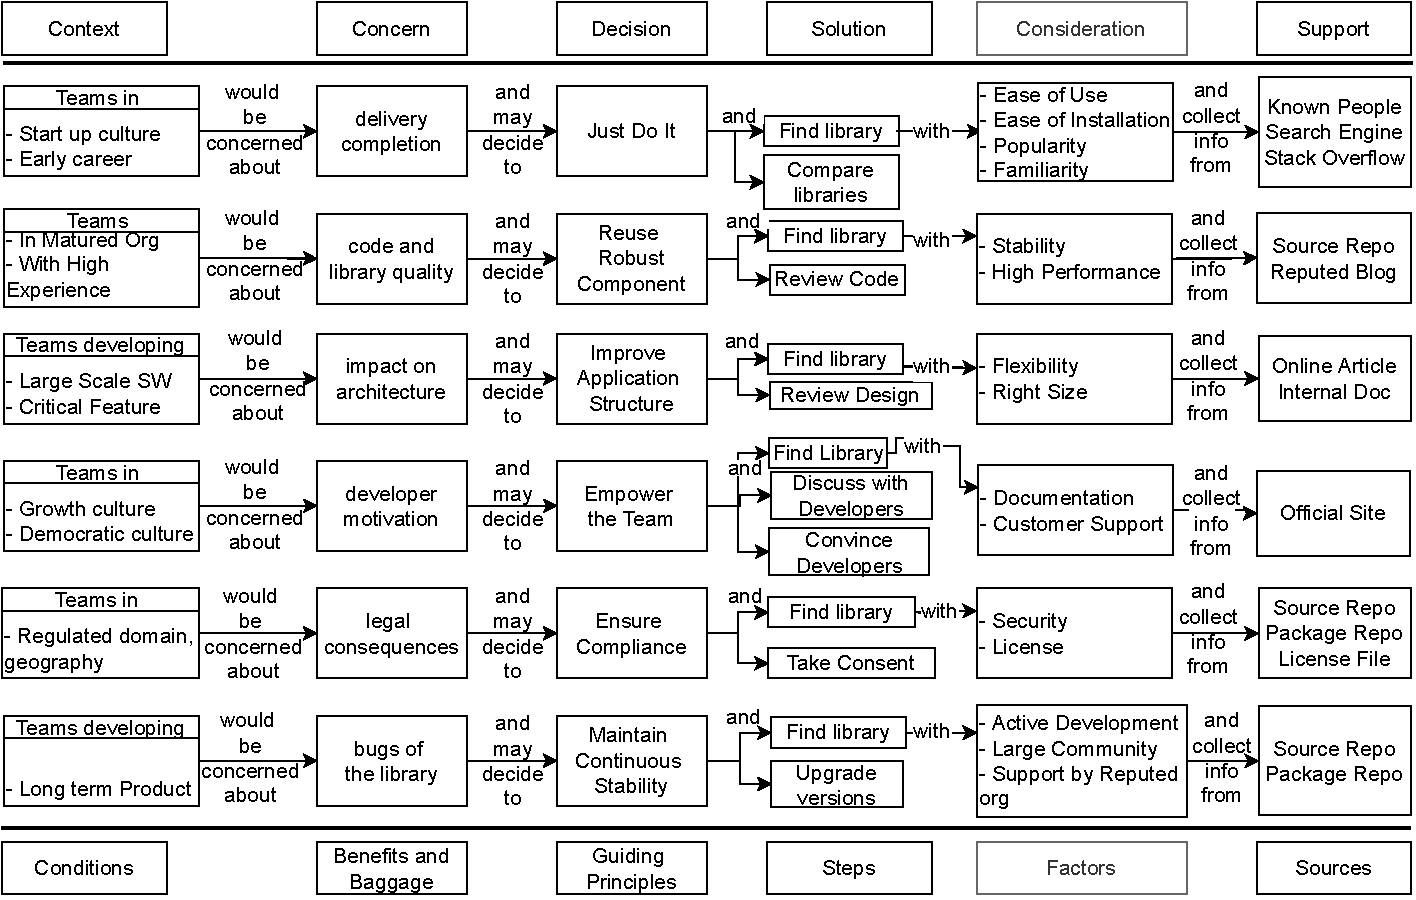
\includegraphics[scale=0.75]{images/gp-concepts-2.pdf}
%    \caption{Interaction of guiding principles with library adoption process %concepts according to the conceptual framework}
%    \label{fig:gp-scneraios}
%\end{figure*}




